\documentclass[%
 %reprint,
  twocolumn,
 %superscriptaddress,
 %groupedaddress,
 %unsortedaddress,
 %runinaddress,
 %frontmatterverbose,
 % preprint,
 showpacs,
 showkeys,
 preprintnumbers,
 %nofootinbib,
 %nobibnotes,
 %bibnotes,
 amsmath,amssymb,
 aps,
 % prl,
  pra,
 % prb,
 % rmp,
 %prstab,
 %prstper,
  longbibliography,
 floatfix,
 %lengthcheck,%
 ]{revtex4-1}

\usepackage{tikz}
\usetikzlibrary{decorations.pathreplacing,decorations.markings}


\tikzset{
  % style to apply some styles to each segment of a path
  on each segment/.style={
    decorate,
    decoration={
      show path construction,
      moveto code={},
      lineto code={
        \path [#1]
        (\tikzinputsegmentfirst) -- (\tikzinputsegmentlast);
      },
      curveto code={
        \path [#1] (\tikzinputsegmentfirst)
        .. controls
        (\tikzinputsegmentsupporta) and (\tikzinputsegmentsupportb)
        ..
        (\tikzinputsegmentlast);
      },
      closepath code={
        \path [#1]
        (\tikzinputsegmentfirst) -- (\tikzinputsegmentlast);
      },
    },
  },
  % style to add an arrow in the middle of a path
  mid arrow/.style={postaction={decorate,decoration={
        markings,
        mark=at position .5 with {\arrow[#1]{stealth}}
      }}},
 % style to add an arrow in 1/4th of a path
  oneforth arrow/.style={postaction={decorate,decoration={
        markings,
        mark=at position .25 with {\arrow[#1]{stealth}}
      }}},
 % style to add an arrow in 1/4th of a path
  threeforth arrow/.style={postaction={decorate,decoration={
        markings,
        mark=at position .75 with {\arrow[#1]{stealth}}
      }}},
}
\begin{document}
\begin{center}
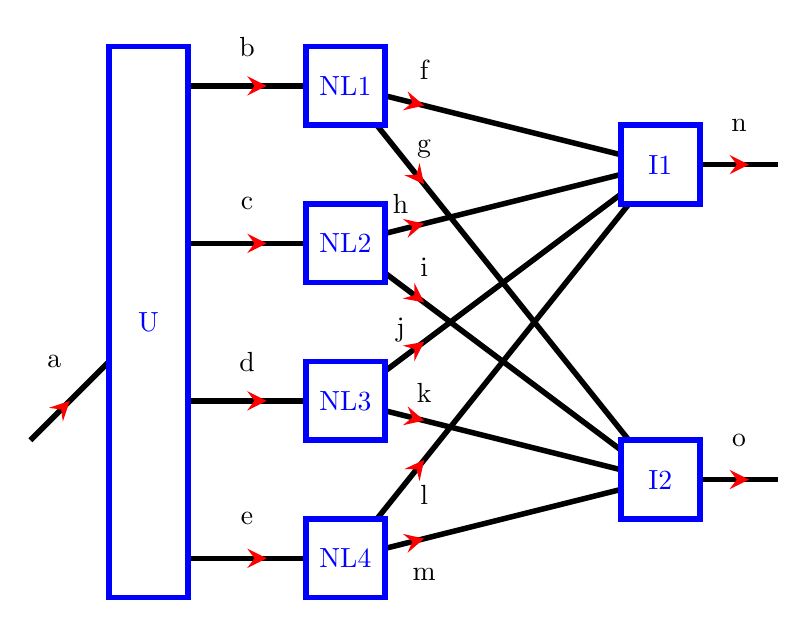
\begin{tikzpicture} [scale=1]

\tikzstyle{every path}=[line width=2pt]

 \path
  (0,2) coordinate(1)
  (2,4) coordinate(2)  % U
  (2,6.5) coordinate(11)  % U
  (2,4.5) coordinate(12)  % U
  (2,2.5) coordinate(13)  % U
  (2,0.5) coordinate(14)  % U
  (4,6.5) coordinate(3)  % NL4
  (4,4.5) coordinate(4)  % NL3
  (4,2.5) coordinate(5)  % NL2
  (4,0.5) coordinate(6)  % NL1
  (8,5.5) coordinate(7)  % I1
  (8,1.5) coordinate(8)  % I2
  (9.5,5.5) coordinate(9)  % n
  (9.5,1.5) coordinate(10)  % o
;


\path [draw=black,postaction={on each segment={oneforth arrow=red}}]  (1) -- (2) ;

\path [draw=black,postaction={on each segment={mid arrow=red}}]  (11) -- (3);
\path [draw=black,postaction={on each segment={mid arrow=red}}]  (12) -- (4);
\path [draw=black,postaction={on each segment={mid arrow=red}}]  (13) -- (5);
\path [draw=black,postaction={on each segment={mid arrow=red}}]  (14) -- (6);

\path [draw=black,postaction={on each segment={oneforth arrow=red}}]  (3) -- (7);
\path [draw=black,postaction={on each segment={oneforth arrow=red}}]  (3) -- (8);
\path [draw=black,postaction={on each segment={oneforth arrow=red}}]  (4) -- (7);
\path [draw=black,postaction={on each segment={oneforth arrow=red}}]  (4) -- (8);
\path [draw=black,postaction={on each segment={oneforth arrow=red}}]  (5) -- (7);
\path [draw=black,postaction={on each segment={oneforth arrow=red}}]  (5) -- (8);
\path [draw=black,postaction={on each segment={oneforth arrow=red}}]  (6) -- (7);
\path [draw=black,postaction={on each segment={oneforth arrow=red}}]  (6) -- (8);

\path [draw=black,postaction={on each segment={threeforth arrow=red}}]  (7) -- (9);
\path [draw=black,postaction={on each segment={threeforth arrow=red}}]  (8) -- (10);

\draw [blue,fill=white] (2) ++(-1,-4) rectangle node {U} ++(1,7);
\draw [blue,fill=white] (3) ++(-0.5,-0.5) rectangle node {NL1} ++(1,1);
\draw [blue,fill=white] (4) ++(-0.5,-0.5) rectangle node {NL2} ++(1,1);
\draw [blue,fill=white] (5) ++(-0.5,-0.5) rectangle node {NL3} ++(1,1);
\draw [blue,fill=white] (6) ++(-0.5,-0.5) rectangle node {NL4} ++(1,1);
\draw [blue,fill=white] (7) ++(-0.5,-0.5) rectangle node {I1} ++(1,1);
\draw [blue,fill=white] (8) ++(-0.5,-0.5) rectangle node {I2} ++(1,1);

\node (a) at (0.3,3) {a};
\node (b) at (2.75,7) {b};
\node (c) at (2.75,5) {c};
\node (d) at (2.75,3) {d};
\node (e) at (2.75,1) {e};
\node (f) at (5,6.7) {f};
\node (g) at (5,5.7) {g};
\node (h) at (4.7,5) {h};
\node (i) at (5,4.2) {i};
\node (j) at (4.7,3.4) {j};
\node (k) at (5,2.6) {k};
\node (l) at (5,1.3) {l};
\node (m) at (5,0.3) {m};
\node (n) at (9,6) {n};
\node (o) at (9,2) {o};

\end{tikzpicture}
\end{center}
\end{document}

\path [draw=blue,dashed]  (9) -- (10);
\draw [blue,fill=white] (3) ++(-0.5,-0.5) rectangle node {NL2} ++(1,1);
\draw [blue,fill=white] (4) ++(-0.5,-0.5) rectangle node {NL1} ++(1,1);
\draw [blue,fill=white] (5) ++(-0.5,-0.5) rectangle node {I1} ++(1,1);
\draw [blue,fill=white] (6) ++(-0.5,-0.5) rectangle node {I2} ++(1,1);
\draw (2) coordinate[label=100:BS];

 \path [draw=blue,postaction={on each segment={mid arrow=red}}]
  (.2,0) -- (3,1) arc (0:180:1.4 and 1) -- cycle
  (4,1) circle(.8)
  (6,1) ellipse(.5 and 1)
  (0,3) to [bend left] (3,4)
  (4,3) rectangle (6,4)
  ;
